% DYSLEXIA SWITCH
\newif\ifdys
		
				% ENABLE or DISABLE font change
				% use XeLaTeX if true
				\dystrue
				\dysfalse


\ifdys

\documentclass[a4paper, 14pt]{extarticle}
\usepackage{amsmath,amsfonts,amsthm,amssymb,mathtools}

\tracinglostchars=3 % Report an error if a font does not have a symbol.
\usepackage{fontspec}
\usepackage{unicode-math}
\defaultfontfeatures{ Ligatures=TeX,
                      Scale=MatchUppercase }

\setmainfont{OpenDyslexic}[Scale=1.0]
\setmathfont{Fira Math} % Or maybe try KPMath-Sans?
\setmathfont{OpenDyslexic Italic}[range=it/{Latin,latin}]
\setmathfont{OpenDyslexic}[range=up/{Latin,latin,num}]

\else

\documentclass[a4paper, 12pt]{extarticle}

\usepackage[utf8x]{inputenc}
%fonts
\usepackage{amsmath,amsfonts,amsthm,amssymb,mathtools}
% comment below to default to computer modern
\usepackage{libertinus,libertinust1math}

\fi


\usepackage[french]{babel}
\usepackage[
a4paper,
margin=2cm,
nomarginpar,% We don't want any margin paragraphs
]{geometry}
\usepackage{icomma}

\usepackage{fancyhdr}
\usepackage{array}
\usepackage{hyperref}

\usepackage{multicol, enumerate}
\newcolumntype{P}[1]{>{\centering\arraybackslash}p{#1}}


\usepackage{stackengine}
\newcommand\xrowht[2][0]{\addstackgap[.5\dimexpr#2\relax]{\vphantom{#1}}}

% theorems

\theoremstyle{plain}
\newtheorem{theorem}{Th\'eor\`eme}
\newtheorem*{sol}{Solution}
\theoremstyle{definition}
\newtheorem{ex}{Exercice}
\newtheorem*{rpl}{Rappel}
\newtheorem{enigme}{Énigme}

% corps
\usepackage{calrsfs}
\newcommand{\C}{\mathcal{C}}
\newcommand{\R}{\mathbb{R}}
\newcommand{\Rnn}{\mathbb{R}^{2n}}
\newcommand{\Z}{\mathbb{Z}}
\newcommand{\N}{\mathbb{N}}
\newcommand{\Q}{\mathbb{Q}}

% variance
\newcommand{\Var}[1]{\text{Var}(#1)}

% domain
\newcommand{\D}{\mathcal{D}}


% date
\usepackage{advdate}
\AdvanceDate[0]


% plots
\usepackage{pgfplots}

% table line break
\usepackage{makecell}
%tablestuff
\def\arraystretch{2}
\setlength\tabcolsep{15pt}

%subfigures
\usepackage{subcaption}

\definecolor{myg}{RGB}{56, 140, 70}
\definecolor{myb}{RGB}{45, 111, 177}
\definecolor{myr}{RGB}{199, 68, 64}

% fake sections with no title to move around the merged pdf
\newcommand{\fakesection}[1]{%
  \par\refstepcounter{section}% Increase section counter
  \sectionmark{#1}% Add section mark (header)
  \addcontentsline{toc}{section}{\protect\numberline{\thesection}#1}% Add section to ToC
  % Add more content here, if needed.
}


% SOLUTION SWITCH
\newif\ifsolutions
				\solutionstrue
				%\solutionsfalse

\ifsolutions
	\newcommand{\exe}[2]{
		\begin{ex} #1  \end{ex}
		\begin{sol} #2 \end{sol}
	}
\else
	\newcommand{\exe}[2]{
		\begin{ex} #1  \end{ex}
	}
	
\fi


% tableaux var, signe
\usepackage{tkz-tab}


%pinfty minfty
\newcommand{\pinfty}{{+}\infty}
\newcommand{\minfty}{{-}\infty}

\begin{document}


\usepackage{minted}

\AdvanceDate[0]

\begin{document}
\pagestyle{fancy}
\fancyhead[L]{Seconde}
\fancyhead[C]{\textbf{Représenter des points dans le plan en Python}}
\fancyhead[R]{\today}

Le but de ce document est d'automatiser l'exercice \ref{exe:milieu-segment} de la feuille « Plan cartésien » à l'aide de Python.
Automatiser permet d'accélérer la vitesse de calcul en évitant les erreurs (en ignorant les erreurs probables du programmeur débutant).

\setcounter{Exercise}{9}
\exe{}{
	Représenter les points $A(1;1)$ et $B(3;-1)$ dans un repère orthonormé.
	Représenter le point
		\[ \lambda A + (1-\lambda)B, \]
	pour certaines valeurs de $\lambda$ (lu « lambda ») entre 0 et 1.
}{exe:milieu-segment}{}


\setlength\columnsep{30pt}

\subsection*{Stocker et afficher un nombre}

\begin{multicols}{3}
	\noindent
	Lorsqu'on écrit \texttt{x=0.5}, la valeur à droite du signe « = » est stockée dans la variable à gauche.
	%\columnbreak
	
	\noindent
	La fonction \texttt{print(x)} permet d'afficher la valeur de la variable \texttt{x}.

	\columnbreak
	\centering
	\begin{minipage}{.1\textwidth}
	\python{print}
	\end{minipage}
\end{multicols}

\warning Il faut utiliser le point à la place de la virgule pour séparer la partie décimale de la partie entière des nombres.

\warning Le signe « = » a un sens différent qu'en mathématiques. Il sert uniquement à stocker la valeur de droite dans la variable de gauche.


\subsection*{Définir et stocker une liste de nombres}

\begin{multicols}{2}
	Une liste de nombres est créée avec des crochets. Les éléments sont séparés par des virgules.

	%Le signe « = » stocke la liste à droite dans la variable à gauche.
	\columnbreak
	\centering
	\begin{minipage}{.2\textwidth}
	\python{list}
	\end{minipage}
\end{multicols}

\subsection*{Parcourir une liste}

\begin{multicols}{2}
	Pour parcourir une liste, on utilise la boucle \texttt{for <variable> in <liste>}.
	Pour chaque élément de la liste, l'élément est stocké dans la variable, et tout le bloc est executé.
	
	\columnbreak
	\centering
	\begin{minipage}{.3\textwidth}
	\python{boucle}
	\end{minipage}
\end{multicols}

L'\textbf{indentation} (décalage par ajout d'espaces vides) est importante en Python car elle définit quelles lignes appartiennent ou non au bloc executé à chaque itération de la boucle.
On utilise la touche de tabulation \textbf{Tab} à gauche du clavier pour ajouter ces espaces vides (ou on appuie 4 fois sur la touche espace).

\subsection*{Multiplication est addition}

\begin{multicols}{2}
	Le signe \texttt{+} est utilisé pour l'addition.
	Le signe \texttt{*} est utilisé pour la multiplication.
	
	L'ordre d'opérations et les parenthèses sont pareil qu'en mathématiques.
	
	\columnbreak
	\centering
	\begin{minipage}{.1\textwidth}
	\python{operations}
	\end{minipage}
\end{multicols}

\newpage

\subsection*{Représentation dans un repère}

La librairie \texttt{matplotlib} est utile pour grapher des courbes et des points.

\begin{multicols}{2}
	La première ligne importe la librairie et la nomme \texttt{plt}.
	La deuxième ligne ajoute le point $(3 ; 4)$.
	La troisième ligne affiche le repère dans une nouvelle fenêtre.
	
	\columnbreak
	\centering
	\begin{minipage}{.3\textwidth}
	\python{scatter}
	\end{minipage}
\end{multicols}

\subsection*{Enregistrer le repère obtenu}

\vspace{10cm}

\subsection*{Améliorations possibles}

Quelques améliorations possibles sont proposées avec des exemples d'implémentation.
\begin{multicols}{2}
	\begin{itemize}
		\item Ajouter un quadrillage au repère.
		\item Centrer les axes des abscisses et des ordonnées.
		\item Ajuster la fenêtre en définissant les $x$ et $y$ affichés.
		\item Changer la couleur du point en fonction de la valeur de $\lambda$.
	\end{itemize}
	\vfill\null
	
	\columnbreak
	\centering
	\begin{minipage}{.3\textwidth}
	\python{ameliorations}
	\end{minipage}
\end{multicols}

%%%%%%%%%%%

\newpage
\fancyhead[C]{\textbf{Solutions}}


\setlength\columnsep{-100pt}
\begin{multicols}{2}
	\python{segment}
	
	\columnbreak
	\centering
	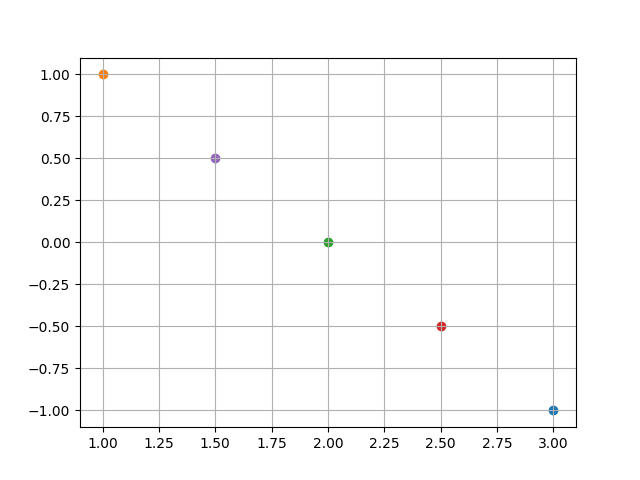
\includegraphics[scale=.7]{segment.png}
\end{multicols}
\hrule
\begin{multicols}{2}
	\python{segment-ameliore}
	\columnbreak
	\centering
	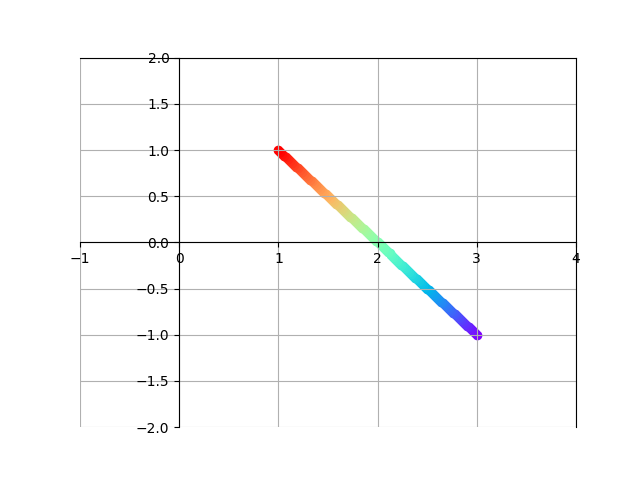
\includegraphics[scale=.7]{segment-ameliore.png}
\end{multicols}

\end{document}
